
%----------------------------------------------------------------------------------------
%	CHAP introduction
%----------------------------------------------------------------------------------------

\chapterimage{blue-chapter-head_4-reduced.pdf} % Chapter heading image

\chapter{Extending MetaR}\label{chap:ExtendingMetaR}

\section{Overview}
Because MetaR is developed in the MPS language workbench, you can use language composition as a way to extend the MetaR language. In this Chapter, we provide a very simple example to illustrate how to extend MetaR through language composition. 


Let's assume that you have just learned about the \texttt{heatmap.2} function provided in the \texttt{gplots} R package. You wish to use this function to create heatmaps with MetaR. To achieve this, you would follow the following steps: 
\begin{enumerate}
\item Create a new MPS Language.
  \item Create a \texttt{Heatmap.2} language concept in the Structure Aspect of the language (see~\cite{campagne2014mps}).
  \item Customize the Generator to transform instances of the \texttt{Heatmap.2} into R code.
\end{enumerate}

\section{Create a new Language}
Let's create a new language. To do this, select the project and do \menu{right-click>New>Language}. Name the language something like \texttt{your.domain.heatmap}.When the language has been created, select its name under the Project Tab and adjust Dependencies to include \textit{org.campagnelab.metaR.tables}. Set the Scope to Extend (this will allow statements of this new language to extend concepts of \textit{org.campagnelab.metaR.tables}). 

\section{Create a new Language Concept}
Select the Structure Aspect of the \textit{your.domain.heatmap} language and do \menu{right-click>New >Concept}. Name the concept \texttt{Heatmap2}. Define the extends clause to be \texttt{Statement} (from language \textit{org.campagnelab.metar.tables}). The resulting concept should appear as shown in Figure~\ref{fig:Heatmap2Concept}.

\paragraph{concept alias}
Define the alias of the concept. Use \texttt{heatmap2}. An instance of the concept will be created when you type this keyword in the editor. 

\paragraph{reference to a table}
To plot a heatmap, we will take data from a MetaR table. This can be achieved by adding a TableRef child to the \texttt{Heatmap2} concept.
\paragraph{heatmap produces a plot}
The heatmap2 statement will produce a plot, so you need to add a child of type \texttt{Plot}. You may call this child `plot' for simplicity.

\begin{figure}[htbp]
  \centering
  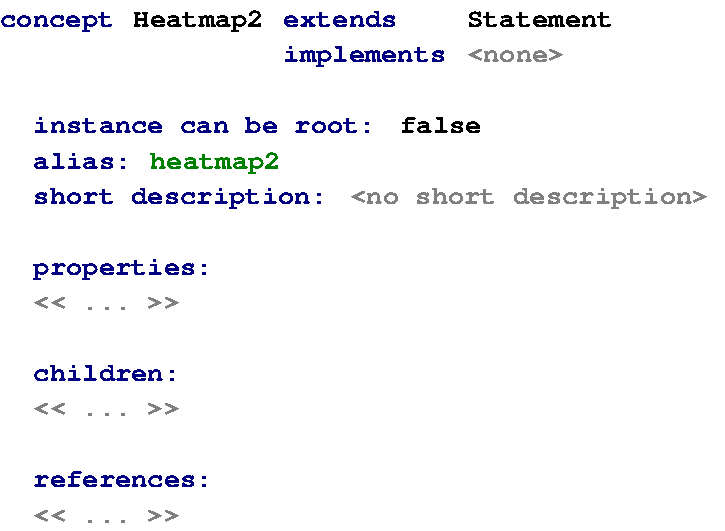
\includegraphics[width=\figWidthNarrow]{figures/Heatmap2Concept.pdf}
\caption[Heatmap2 Concept.]{\textbf{Heatmap2 Concept.} The Heatmap2 concept extends Statement. When the language is composed with MetaR, Heatmap2 will become available for auto-completion whenever a MetaR Statement can be used.}
\label{fig:Heatmap2Concept}
\end{figure}

\section{Define the Editor}
An MPS editor customizes how a node appears in the editor. Create an editor for \texttt{Heatmap2} (see~\cite{campagne2014mps}) and define its content as shown in Figure~\ref{fig:EditorForHeatmap2}.
\begin{SCfigure}
  \centering
  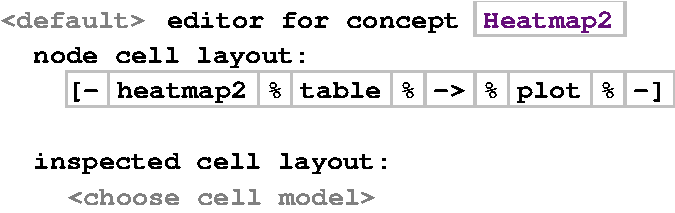
\includegraphics[width=\figWidthNarrow]{figures/EditorForHeatmap2.pdf}
\caption[Editor of the Heatmap2 Statement.]{\textbf{Editor of the Heatmap2 Statement.} Notice how the editor simply shows the name of the statement, delegates to the TableRef editor to render the table reference, and delegates to the Plot editor to show the plot child.}
\label{fig:EditorForHeatmap2}
\end{SCfigure}

\section{Generate R Code}

